\documentclass[11pt]{article}

% ==== PACKAGES ==== %
% \usepackage{fullpage}
\usepackage{amsmath,amssymb,amsthm}
\usepackage{epic}
\usepackage{eepic}
\usepackage{hyperref}
\usepackage{listings}
\usepackage{float}
\usepackage{graphicx}
\usepackage{fancyhdr}
\usepackage{color}
\usepackage{bbm}
\usepackage[letterpaper, margin=1in]{geometry}

% ==== MARGINS ==== %
% \pagestyle{empty}
% \setlength{\oddsidemargin}{0in}
% \setlength{\textwidth}{6.8in}
% \setlength{\textheight}{9.5in}

\pagestyle{fancy}
\fancyhf{}
\rhead{ASEN 5044}
\lhead{Midterm 1}
\rfoot{Page \thepage}


\newtheorem*{solution*}{Solution}
\newtheorem{lemma}{Lemma}[section]
\newtheorem{theorem}[lemma]{Theorem}
\newtheorem{claim}[lemma]{Claim}
\newtheorem{definition}[lemma]{Definition}
\newtheorem{corollary}[lemma]{Corollary}
\lstset{moredelim=[is][\bfseries]{[*}{*]}}

% ==== DOCUMENT PROPER ==== %
\begin{document}

\thispagestyle{empty}

% --- Header Box --- %
\newlength{\boxlength}\setlength{\boxlength}{\textwidth}
\addtolength{\boxlength}{-4mm}

\begin{center}\framebox{\parbox{\boxlength}{\bf
      Statistical Estimation \hfill Midterm 1\\
      ASEN 5044 Fall 2018 \hfill Due Date: Oct 11, 2018\\
      Name: Andrew Kramer \hfill PhD Student
}}
\end{center}

\section*{Problem 1}
Inverted pendulum with equations of motion:
\begin{align*}
	(M+m)\ddot{z}-ml\ddot{\theta}\cos\theta&+ml\dot{\theta}^2\sin\theta=P \\
	l\ddot{\theta}-g\sin\theta &= \ddot{z}\cos\theta
\end{align*}
\subsection*{Part (a)}

The system's state equations can be expressed as follows:
\begin{equation*}
	\dot{x} = \begin{bmatrix} \dot{x}_1 \\ \dot{x}_2 \\ \dot{x}_3 \\ \dot{x}_4 \end{bmatrix} = \begin{bmatrix} f_1(x,u,t) \\ f_2(x,u,t) \\ f_3(x,u,t) \\ f_4(x,u,t) \end{bmatrix} = \begin{bmatrix} x_2 \\ \frac{P-g\sin x_3 \cos x_3-mlx_4^2\sin x_3}{M+m\sin^2x_3} \\ x_4 \\ \frac{P\cos x_3 - mlx_4^2\sin x_3 \cos x_3 + (M+m)g\sin x_3}{Ml + ml\sin^2x_3} \end{bmatrix}
\end{equation*}
To demonstrate the system is in equilibrium at $\dot{z}=0,\ \theta=0,\ \dot{\theta}=0$, and $P(t)=0$ we note first that at the given conditions the equations of motion become 
\begin{align*}
	(M+m)\ddot{z}-ml\ddot{\theta} &= 0 \\
	l\ddot{\theta} &= \ddot{z}
\end{align*}
If we plug the second equation back into the first we get
\begin{equation*}
	(M+m)\ddot{z} - m\ddot{z}=M\ddot{z}=0
\end{equation*}
Because we know $M$ is not equal to zero, this means $\ddot{z}$ must be equal to zero. Additionally, because $\ddot{z} = l\ddot{\theta}$ and $l\neq0$ we can also conclude that $\ddot{\theta}=0$. This means $\dot{x}=0$ under the given conditions and the system is therefore in equilibrium.

\subsection*{Part (b)}
We'll noting that our measurement function in state space form is
\begin{equation*}
	y = h(x,u,t) = x_1 - l\sin x_3
\end{equation*}
Next we define $\tilde{x}$, $\tilde{y}y$, and $\tilde{u}$ where $\tilde{x}(t) = x(t) - x_\text{nom}(t)$, and $\tilde{y}$ and $\tilde{u}$ are defined similarly. We can then find $A|_\text{nom}$, $B|_\text{nom}$, $C|_\text{nom}$, and $D|_\text{nom}$ such that 
\begin{align*}
	\dot{\tilde{x}} &= A|_\text{nom}\tilde{x}(t) + B|_\text{nom}\tilde{u}(t) \\
	\tilde{y} &= C|_\text{nom}\tilde{x}(t) + D|_\text{nom}\tilde{u}(t)
\end{align*} 
The above matrices are defined as
\begin{align*}
	A|_\text{nom} &= \frac{\partial f}{\partial x} \Bigg|_\text{nom}\quad B|_\text{nom} = \frac{\partial f}{\partial u} \Bigg|_\text{nom} \\
	C|_\text{nom} &= \frac{\partial h}{\partial x} \Bigg|_\text{nom}\quad D|_\text{nom} = \frac{\partial h}{\partial u}\Bigg|_\text{nom}
\end{align*}
The jacobians are as follows
\begin{align*}
	\frac{\partial f}{\partial x} &= \begin{bmatrix} 0&1&0&0 \\ 0&0&\frac{\partial f_2}{\partial x_3}&\frac{\partial f_2}{\partial x_4} \\ 0&0&0&1 \\ 0&0&\frac{\partial f_4}{\partial x_3}&\frac{\partial f_4}{\partial x_4}\end{bmatrix} \\
	\frac{\partial f}{\partial u} &= \begin{bmatrix} 0 \\ \frac{1}{M+m\sin^2x_3} \\ 0 \\ \frac{\cos x_3}{Ml + ml \sin^2x_3} \end{bmatrix} \\
	\frac{\partial h}{\partial x} &= \begin{bmatrix} 1&0&-l\cos x_3&0\end{bmatrix} \\
	\frac{\partial h}{\partial u} &= [0]
\end{align*}
where
\begin{align*}
	\frac{\partial f_2}{\partial x_3} &= \frac{-2m(P-g\sin x_3\cos x_3-lmx_4^2\sin x_3)\sin x_3 \cos x_3}{(M+m\sin^2x_3)^2} + \frac{g\sin^2x_3 - g\cos^2x_3 - lmx_4^2\cos x_3}{M+m\sin^2x_3} \\
	\frac{\partial f_2}{\partial x_4} &= -\frac{2lmx_4\sin x_3}{M+m\sin^2x_3} \\
	\frac{\partial f_4}{\partial x_3} &= \frac{-2lm(P\cos x_3 + g(M+m)\sin x_3 - lmx_4^2\sin x_3 \cos x_3)\sin x_3 \cos x_3}{(Ml + ml\sin^2x_3)^2} \\ &\qquad + \frac{-P\sin x_3 + g(M+m)\cos x_3 + lmx_4^2\sin^2x_3 - lmx_4^2\cos^2x_3}{Ml + ml\sin^2x_3} \\
	\frac{\partial f_4}{\partial x_4} &= -\frac{2mlx_4\sin x_3 \cos x_3}{ML + ml\sin^2x_3}
\end{align*}
When these jacobians are evaluated at $x_\text{nom}$, $u_\text{nom}$ we get the following matrices our linearized state-space equations:
\begin{align*}
	A|_\text{nom} &= \begin{bmatrix} 
					0 & 1 & 0 & 0 \\ 
					0 & 0 & 2m-\frac{g}{m} & 0 \\
					0 & 0 & 0 & 1 \\ 
					0 & 0 & \frac{g(M+m)}{Ml} & 0 \end{bmatrix} \\
	B|_\text{nom} &= \begin{bmatrix} 
					0 \\ \frac{1}{M} \\ 0 \\ \frac{1}{Ml} 
					\end{bmatrix} \\
	C|_\text{nom} &= \begin{bmatrix}
					1 & 0 & -1 & 0 \end{bmatrix} \\
	D|_\text{nom} &= [0]
\end{align*}

\subsection*{Part (c)}
\subsection*{Part (d)}
\subsection*{Part (e)}
\subsection*{Part (f)}
\subsection*{Part (g)}
\section*{Problem 2}
Two 6-sided dice rolls with $R_1$ and $R_2$ denoting the outcome of the first and second die, respectively.

\subsection*{Part (a)}
$P(R_1)=P(R_2)=\frac{1}{6}$ for all $R_1$ and $R_2$. Because the outcomes $R_1$ and $R_2$ are independent, $P(R_1,R_2)=P(R_1)*P(R_2)$. So
\begin{equation*}
	P(R_1,R_2)=\frac{1}{36},\ \forall R_1,R_2
\end{equation*}

\subsection*{Part (b)}
The joint probabilities for $X$ and $Y$ are shown in table \ref{joints} below
\begin{table}[h!]
  \begin{center}
    \caption{Joint Probabilities}
    \label{joints}
    \begin{tabular}{c|c|c|c|c|c|c} % <-- Alignments: 1st column left, 2nd middle and 3rd right, with vertical lines in between
      X & Y=1 & Y=2 & Y=3 & Y=4 & Y=5 & Y=6 \\
      \hline
      1 & 1/36 & 2/36 & 2/36 & 2/36 & 2/36 & 2/36 \\
      2 & 0 & 1/36 & 2/36 & 2/36 & 2/36 & 2/36 \\
      3 & 0 & 0 & 1/36 & 2/36 & 2/36 & 2/36 \\
      4 & 0 & 0 & 0 & 1/36 & 2/36 & 2/36 \\
      5 & 0 & 0 & 0 & 0 & 1/36 & 2/36 \\
      6 & 0 & 0 & 0 & 0 & 0 & 1/36 \\
    \end{tabular}
  \end{center}
\end{table}

\subsection*{Part (c)}
The marginal probabilities of $X$ obtained from the sum $\sum_yP(X=x,Y=y)$
and the marginal probabilities of $Y$ obtained from the sum $\sum_xP(X=x,Y=y)$ are shown below in table \ref{marginals}.
\begin{table}[h!]
  \begin{center}
    \caption{Marginal Probabilities}
    \label{marginals}
    \begin{tabular}{c|c|c} % <-- Alignments: 1st column left, 2nd middle and 3rd right, with vertical lines in between
       & X & Y \\
      \hline
      1 & 11/36 & 1/36 \\
      2 & 9/36 & 3/36 \\
      3 & 7/36 & 5/36 \\
      4 & 5/36 & 7/36 \\
      5 & 3/36 & 9/36 \\
      6 & 1/36 & 11/36 \\
    \end{tabular}
  \end{center}
\end{table}

\subsection*{Part (d)}
$X$ and $Y$ are not independent. Two variables are considered independent if the realization of one variable does not affect the probability of the other. This is not the case for $X$ and $Y$. By the definitions of $X$ and $Y$, the value of $Y$ cannot be less than the value of $X$, since the maximum of $R_1$ and $R_2$ cannot be less than the minimum. So the $P(Y=3,X=5)=0$, while $P(Y=3,X=1) = 2/36$.

\section*{Problem 3}
A random variable $X$ has the pdf $p(x)=k(1-x^4)$ for $-1\leq x\leq1$ and $p(x)=0$ elsewhere.

\subsection*{Part (a)}
Because $\int_{-\infty}^\infty p(x)dx = 1$ we can find $k$ as follows:
\begin{align*}
	\int_{-1}^1 k(1-x^4)dx &= 1 \\
	k\int_{-1}^1(1-x^4)dx &= \\
	k \big[x-\frac{1}{5}x^5 \big|_{-1}^1 &= \\
	k\Big(1-\frac{1}{5}+1-\frac{1}{5}\Big) &= \\
	\frac{8k}{5} &= 1 \\
	k = \frac{5}{8}
\end{align*}
Now we can calculate $E[x] = \int_{-\infty}^\infty xp(x)dx$ as follows:
\begin{align*}
	\int_{-\infty}^\infty xp(x)dx &= \frac{5}{8}\int_{-1}^1x(1-x^4)dx \\
	&= \frac{5}{8}\int_{-1}^1(x-x^5)dx \\
	&= \frac{5}{8} \Bigg[\frac{1}{2}x^2 - \frac{1}{6}x^6 \Bigg|_{-1}^1 \\
	&= \frac{5}{8} \Bigg(\frac{1}{2} - \frac{1}{6} - \frac{1}{2} + \frac{1}{6}\Bigg) \\
	&= 0
\end{align*}
Next we find $E[x^2] = \int_{-\infty}^\infty x^2p(x)dx$ as
\begin{align*}
	\int_{-\infty}^\infty x^2p(x)dx &= \frac{5}{8}\int_{-1}^1x^2(1-x^4)dx \\
	&= \frac{5}{8}\int_{-1}^1(x^2-x^6)dx \\
	&= \frac{5}{8} \Bigg[\frac{1}{3}x^3 - \frac{1}{7}x^7 \Bigg|_{-1}^1 \\
	&= \frac{5}{8} \Bigg(\frac{1}{3} - \frac{1}{7} + \frac{1}{3} - \frac{1}{7}\Bigg) \\
	&= \frac{5}{21}
\end{align*}
Finally we can find $\text{var}(x) = E[x^2]-(E[x])^2 = \frac{5}{21}-0=\frac{5}{21}$.

\subsection*{Part (b)}
The cumulative distribution function is defined as $P_X(\zeta)=\int_{-\infty}^\zeta p(x)dx$. So the cdf is:
\begin{align*}
	P_X(\zeta)&=\int_{-\infty}^\zeta p(x)dx \\
	&= \frac{5}{8}\int_{-1}^\zeta (1-x^4)dx \\
	&= \frac{5}{8} \Big[x-\frac{1}{5}x^5\Big|_{-1}^\zeta \\
	&= \frac{5}{8} \Big(\zeta - \frac{1}{5}\zeta^5 + \frac{4}{5}\Big)
\end{align*}

\subsection*{Part (c)}
Because the pdf is symmetric about zero, $P(|X| < 0.5)$ is equivalent to $P(-0.5<X<0.5)$, which can be found as
\begin{equation*}
	P(-0.5<X<0.5) = P_X(0.5) - P_X(-0.5) = 0.7895
\end{equation*}

\section*{Problem 4}
Blood alcohol tests on drivers given the conditional probabilities given in table \ref{conditionals}:

\begin{table}[h!]
  \begin{center}
    \caption{Conditional Probabilities}
    \label{conditionals}
    \begin{tabular}{c|c|c} % <-- Alignments: 1st column left, 2nd middle and 3rd right, with vertical lines in between
      $P(T|A)$ & $A=\text{drunk}$ & $A=\text{sober}$ \\
      \hline
      $T=\text{positive}$ & 0.99 & 0.001 \\
      $T=\text{negative}$ & 0.01 & 0.999 \\
    \end{tabular}
  \end{center}
\end{table}

\subsection*{Part (a)}
We can find $P(A=\text{drunk}|T=\text{positive})$ through a straightforward application of Bayes' rule:
\begin{equation*}
	P(A=\text{drunk}|T=\text{positive}) = \frac{P(T=\text{positive}|A=\text{drunk})*P(A=\text{drunk})}{P(T=\text{positive})}
\end{equation*}
Since we aren't given a number for $P(T=\text{positive})$ we can find it as $P(T=\text{positive})=P(T=\text{positive}|A=\text{drunk})P(A=\text{drunk})+P(T=\text{positive}|A=\text{sober})P(A=\text{sober})=0.99*0.2+0.001*0.8=0.1988$. So the conditional probability is:
\begin{equation*}
	P(A=\text{drunk}|T=\text{positive}) = \frac{0.99*0.2}{0.1988} = 0.996
\end{equation*}
\subsection*{Part (b)}
If $P(A=\text{drunk})=0.001$ the probability $P(T=\text{positive})=0.99*0.001+.001*0.999=0.002$. So the conditional probability becomes
\begin{equation*}
	P(A=\text{drunk}|T=\text{positive}) = \frac{0.99*0.001}{0.002} = 0.495
\end{equation*}

\section*{Problem AQ1}
Probability of abiogenesis occurring on an Earth-like planet is given by 
\begin{equation*}
	P(\lambda,n,t)=\text{Poisson}[\lambda,n,t]=e^{-\lambda(t-t_\text{min})}\frac{\{\lambda(t-t_\text{min}\}^n}{n!}
\end{equation*}

\subsection*{Part (a)}
The probability of life arising at least once ($n\geq1$) could be calculated from the infinite sum
\begin{equation*}
	P(\lambda,n\geq1,t)=\sum_{n=1}^\infty P[\lambda,n,t]
\end{equation*}
This sum would be difficult to evaluate, however, and we can make things easier for ourselves by noting that the probability life arises at least once is equivalent to the probability that it doesn't arise zero times. Because $\sum_{n=0}^\infty P(\lambda,n,t)=1$, we can calculate the probability life arises at least once as:
\begin{equation*}
	P(\lambda,n\geq1,t) = 1-P(\lambda,0,t)=1-e^{-\lambda(t-t_\text{min})}\frac{\{\lambda(t-t_\text{min}\}^0}{0!} = 1-e^{-\lambda(t-t_\text{min})}
\end{equation*}

\subsection*{Part (b)}
The probability life arises at least once within $t_\text{emerge}$ is 
\begin{equation*}
	P(E=1)=1-e^{-\lambda(t_\text{emerge}-t_\text{min})}
\end{equation*} 
Similarly, the probability life arises at least once within $t_\text{req}$ is
\begin{equation*}
	P(R=1)=1-e^{-\lambda(t_\text{req}-t_\text{min})}
\end{equation*}
Lastly, because $t_\text{min} < t_\text{emerge} < t_\text{req}$, we know that if life has arisen within $t_\text{emerge}$ then it definitely has also arisen within $t_\text{required}$, so $P(R=1|E=1)=1$. Using these probabilities we can apply Bayes rule to get
\begin{equation*}
	P(E=1|R=1) = \frac{P(R=1|E=1)P(E=1)}{P(R=1)} = \frac{1-e^{-\lambda(t_\text{emerge}-t_\text{min})}}{1-e^{-\lambda(t_\text{req}-t_\text{min})}}
\end{equation*}

\subsection*{Part (c)}
The conditional probability $P(E=1|R=1,\lambda,t_\text{min})$ can be expressed as the following likelihood function given $y=\log_{10}\lambda$:
\begin{equation*}
	P(E=1|R=1,y,t_\text{min})=\frac{1-e^{-(10^y)(t_\text{emerge}-t_\text{min})}}{1-e^{-(10^y)(t_\text{req}-t_\text{min})}}
\end{equation*}
Given this likelihood function, we can find the posterior for $y$ via Bayes' rule
\begin{equation*}
	P(y|E=1,R=1,t_\text{min}) = \frac{P(y)P(E=1|R=1,y,t_\text{min})}{\int_{-\infty}^\infty P(y)P(E=1|R=1,y,t_\text{min})dy}
\end{equation*}
For the given cases, $P(y)$ was replaced with the appropriate density function, $P(E=1|R=1,y,t_\text{min})$ was replaced with the likelihood function given above and $P(y)P(E=1|R=1,y,t_\text{min})$ was evaluated at $10^4$ $y$ values in the range $[-3,3]$. These samples were normalized with the integral $\int_{-\infty}^\infty P(y)P(E=1|R=1,y,t_\text{min})dy$, numerically evaluated using a right Reimann sum over the same range of $y$ values. The posteriors $P(y|R=1,E=1,t_\text{min})$ for cases 1, 2, and 3 are plotted in figures \ref{AQ1_plot1}, \ref{AQ1_plot2}, and \ref{AQ1_plot3}, respectively. On each figure the posterior is plotted in blue, while the likelihood function is plotted in red and the prior is plotted in yellow.
\begin{figure}[h!]
	\centering
	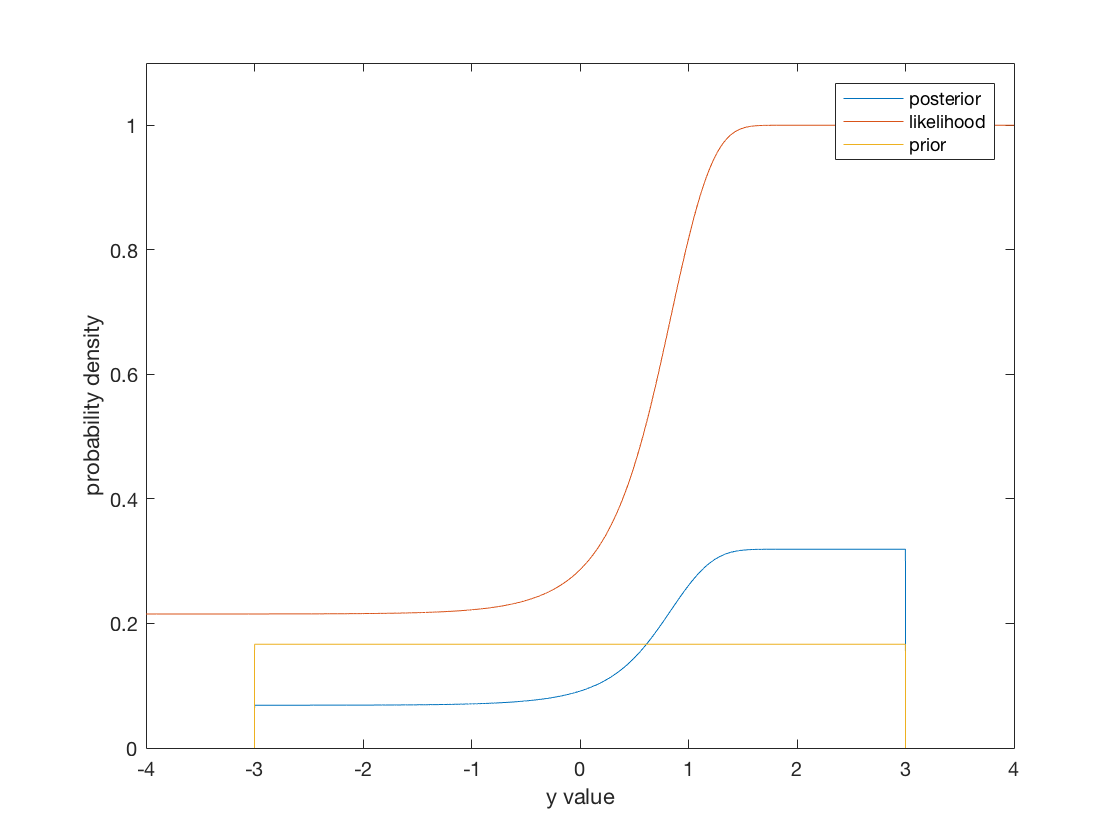
\includegraphics[width=0.6\linewidth]{AQ1_plot1.png}
	\caption{pdfs for case 1}
	\label{AQ1_plot1}
\end{figure}
\begin{figure}[h!]
	\centering
	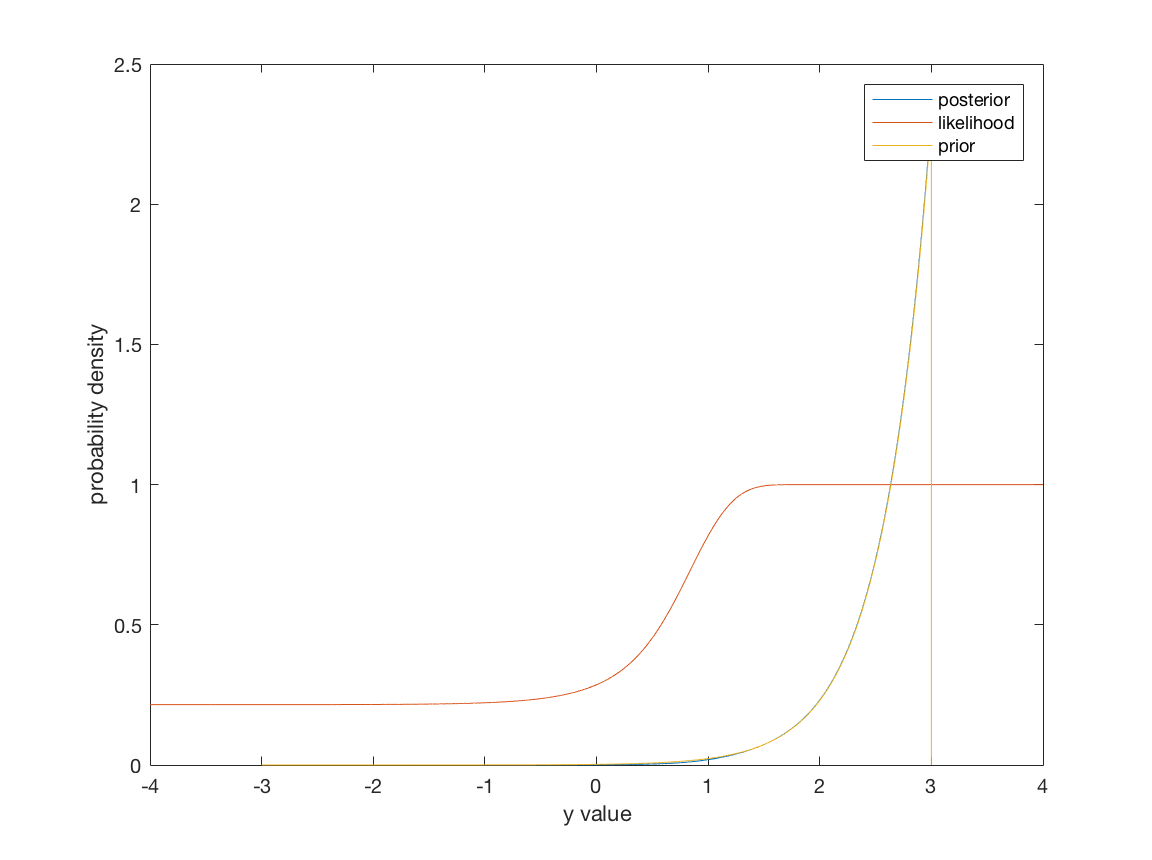
\includegraphics[width=0.6\linewidth]{AQ1_plot2.png}
	\caption{pdfs for case 2}
	\label{AQ1_plot2}
\end{figure}
\begin{figure}[h!]
	\centering
	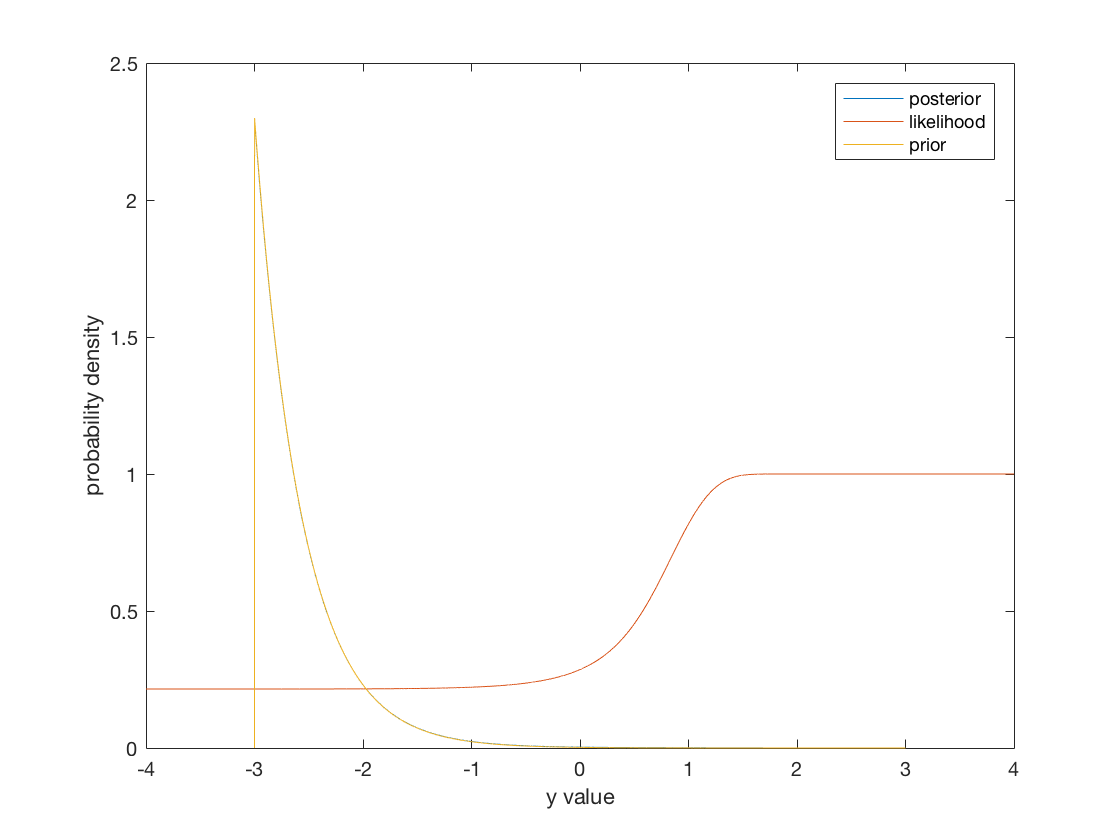
\includegraphics[width=0.6\linewidth]{AQ1_plot3.png}
	\caption{pdfs for case 3}
	\label{AQ1_plot3}
\end{figure}

\subsection*{Part (d)}
Case 1 shows the greatest change from the prior. As can be seen in figures \ref{AQ1_plot2} and \ref{AQ1_plot3}, the prior essentially overrides the likelihood function in cases 2 and 3, and there is little difference between the prior and posterior in these cases. If the intention of conditioning the prior using the likelihood function is to update the prior given information from the likelihood function, then the prior from case 1 is the best. This is because the posterior in case 1 is clearly a fusion of the prior and the likelihood function. In cases 2, and 3, it is difficult to tell that the likelihood function has had any affect at all on the posterior.

\end{document}

